\section{Quantum Entanglement}
La maggior parte degli stati di un sistema ad n-qubit non può essere scritto come il prodotto tensioriale di n qubit singoli, nonostante siano tutte delle combinazioni lineari degli elementi della base del sistema ad n-qubit.

Un caso speciale di superposizione di più qubit è quella in cui non posso scrivere lo stato del mio sistema ad n-qubit come il prodotto tensoriale di questi ultimi. Tali stati sono detti stati entranglati (\textbf{entrangled states}).

\[
\ket{\varphi} \ne \ket{u} \otimes \ket{v}, \ket{u},\ket{v} \text{qubits
}
\]

Per comprendere al meglio tale concetto, considerando un generico sistema di 2 qubit, si avrà che:
\[
\ket{\varphi} = \frac{1}{\sqrt{2}}(\ket{00} + \ket{01})
\]

Tale Qubit può essere riscritto come prodotto tensoriale dei due qubit, come:
\[
\ket{\varphi} = \ket{0} \otimes \frac{1}{\sqrt{2}}(\ket{0} + \ket{1})
\]

Da cui posso ben distinguere lo stato dei due qubit, in maniera del tutto indipendente l'uno dall'altro. Questo, in un certo senso, è come dire che i due qubit, tra di loro, non interagiscono e non dipendono l'uno dall'altro.

Mentre nel caso di un \textbf{entangled state}, si avrà che:

\[
\ket{\varphi} = \ket{\Phi^+} = \frac{1}{\sqrt{2}}(\ket{00} + \ket{11})
\]

Tale stato non può essere decomposto in un prodotto tensoriale tra due Qubit distinti. Questo è spiegato dal fatto, che determinato lo stato di un qubit, sarà automaticamente determinato anche lo stato dell'altro qubit. Questo è un risultato interessante, dato che il sistema sembra essere all'interno di uno stato in cui una eventuale misurazione, e quindi un collasso, sul primo Qubit, autodetermineranno lo stato del secondo qubit. 

Per dimostrare che non sia possibile rappresentare lo stato \(\ket{\Phi^+}\) con un prodotto tensoriale è la seguente:
\[
\ket{\Phi^+} = \ket{u} \otimes \ket{v} = 
\begin{bmatrix}
u_1 v_1 \\
u_1 v_2 \\
u_2 v_2 \\
u_2 v_2
\end{bmatrix}
\implies
\]
\[
\implies
\begin{cases}
u_1 v_1 = \frac{1}{\sqrt{2}} \\
u_1 v_2 = 0 \\
u_2 v_1 = 0 \\
u_2 v_2 = \frac{1}{\sqrt{2}}
\end{cases}
\implies
\begin{cases}
u_1 = 0 \implies u_1 v_1 \ne \frac{1}{\sqrt{2}}\\
or \\
v_2 = 0 \implies u_2 v_2 \ne \frac{1}{\sqrt{2}}
\end{cases}
\]

Il che dimostra che non è possibile scrivere tale stato come un prodotto tensoriale di due stati "indipendenti". 

Oltre allo stato \(\ket{\Phi^+}\) vi sono altri 3 stati (nel caso di sistemi a 2 qubit) di bell possibili. Gli \textbf{stati di Bell} sono:
\begin{itemize}
    \item \(\ket{\Phi^+} = \frac{1}{\sqrt{2}}(\ket{00} + \ket{11})\)
    \item \(\ket{\Phi^-} = \frac{1}{\sqrt{2}}(\ket{00}-\ket{11})\)
    \item \(\ket{\Psi^+} = \frac{1}{\sqrt{2}}(\ket{01}+\ket{10})\)
    \item \(\ket{\Psi^-} = \frac{1}{\sqrt{2}}(\ket{01}-\ket{10})\)
\end{itemize}

Effettuare operazioni unitarie sul singolo qubit non vanno a cambiare l'entanglement che c'è, quello che in realtà succede è il passaggio da uno stato di bell ad un altro. Gli stati di Bell sono puri, ma questo implica che i qubit, singolarmente, non si trovano in uno stato puro (considerandoli singolarmente ed in maniera separata). 


\subsection{Misura degli stati di Bell}
Come detto precedentemente, la misura di un qubit su uno stato di Bell, fa collassare anche l'altro nello stato dettato. Se si misurano entrambi i qubit rispetto lo stesso operatore (stessa base ortonormale di riferimento), allora si otterrà un risultato autodeterminato, in base allo stato di Bell in cui ci troviamo. 

Per capire al meglio, consideriamo lo stato
\[
\ket{\Phi^+} = \frac{1}{\sqrt{2}}(\ket{00} + \ket{11})
\]

Si avranno solo due probabilità:
\[
\mathcal{P}_{00} = \mathcal{P}_{11} = \frac{1}{2}
\]

Dove \(\mathcal{P}_{00}\) è la probabilità che i due qubit, dopo la misura, siano entrambi in \(\ket{0}\), mentre \(\mathcal{P}_{11}\) è la probabilità che entrambi i qubit, dopo la misura, si trovino in \(\ket{1}\).

Questo però vuol dire che se misuro i due qubit lungo lo stesso operatore Z (autovettori della base canonica), allora otterrò lo stesso risultato da entrambe le misure in maniera deterministica, il che dirà che tali qubit sono perfettamente correlati. Misurando lungo altri operatori, considerando sempre lo stato \(\ket{\Phi^+}\), il risultato sarà randomico, ma sempre uguale tra le due misure (se le due misure vengono fatte lungo sempre la stessa base). 

La misura di uno stato entangled, quindi, dipende su quale dei due qubit ho effettuato prima la misura. Il caso in cui le due misure avvengano allo stesso tempo viene escluso, poichè dalla teoria della relatività di Einstein riesco sempre a ricavare una misura che avviene prima di un altra. 

Le coppie di particelle entanglate sono anche chiamate \textbf{coppie EPR}(Einstein-Podolsky-Rosen), misurare uno dei due qubit, cambia istantaneamente dell'altro qubit, facendolo collassare.

\begin{info}
\textbf{Generazione delle coppie EPR}\\
Oggi le coppie EPR sono una delle cose da realizzare più challenging. In particolare per il loro utilizzo a lunghe distanze. Più precisamente, una delle metodologie più usate per generare le coppie EPR è l'\textbf{SPDC} (Spontaneous Parametric Down-Conversion) \cite{anwar2021entangled}, tale sistema prevede una pompa (un laser), che viene sparato attraverso un cristallo non lineare, tale fotone ha una piccola probabilità di dividersi in due fotoni ad energia minore detti \textit{signal} ed \textit{idler} (tale processo è tutto interno al cristallo). \cite{pan2012multiphoton}. Quello che permette a tali fotoni di essere entanglati non è l'interazione che c'è tra i due, ma è bensì la legge di conservazione dell'energia e quella di conservazione dell'impulso. Da qui entra poi in gioco quelli che sono gli stati di bell, ovvero il fatto che i due fotoni possono avere polarizzazioni uguali o polarizzazioni ortogonali.

Solitamente, a grandi distanze, si evita generare sempre delle nuove coppie EPR da distribuire, si preferisce partire da due coppie Entanglate, entanglare a sua volta 2 qubit, portandoli in uno stato di bell, per poi misurarli, qesto farà collassare i due entanglement generati precedentemente, facendo entrare, i qubit non misurati, e mai interagenti, in entanglement tra di loro. Questo farà sì di avere solo 2 fotoni entangled, ma ad una "distanza" maggiore. Il circuito a cui si fa riferimento per l'entanglement swapping è quello mostrato nella figura [\ref{img:ent-swapping}]. Tale circuito va letto da sinistra verso desctra considerando l'avanzata verso destra come il tempo, mentre, le linee continue sono i qubit che evolvono, mentre la doppia linea grigia sono dei bit classici che evolvono nel tempo
\end{info}

\begin{figure}[H]
\centering
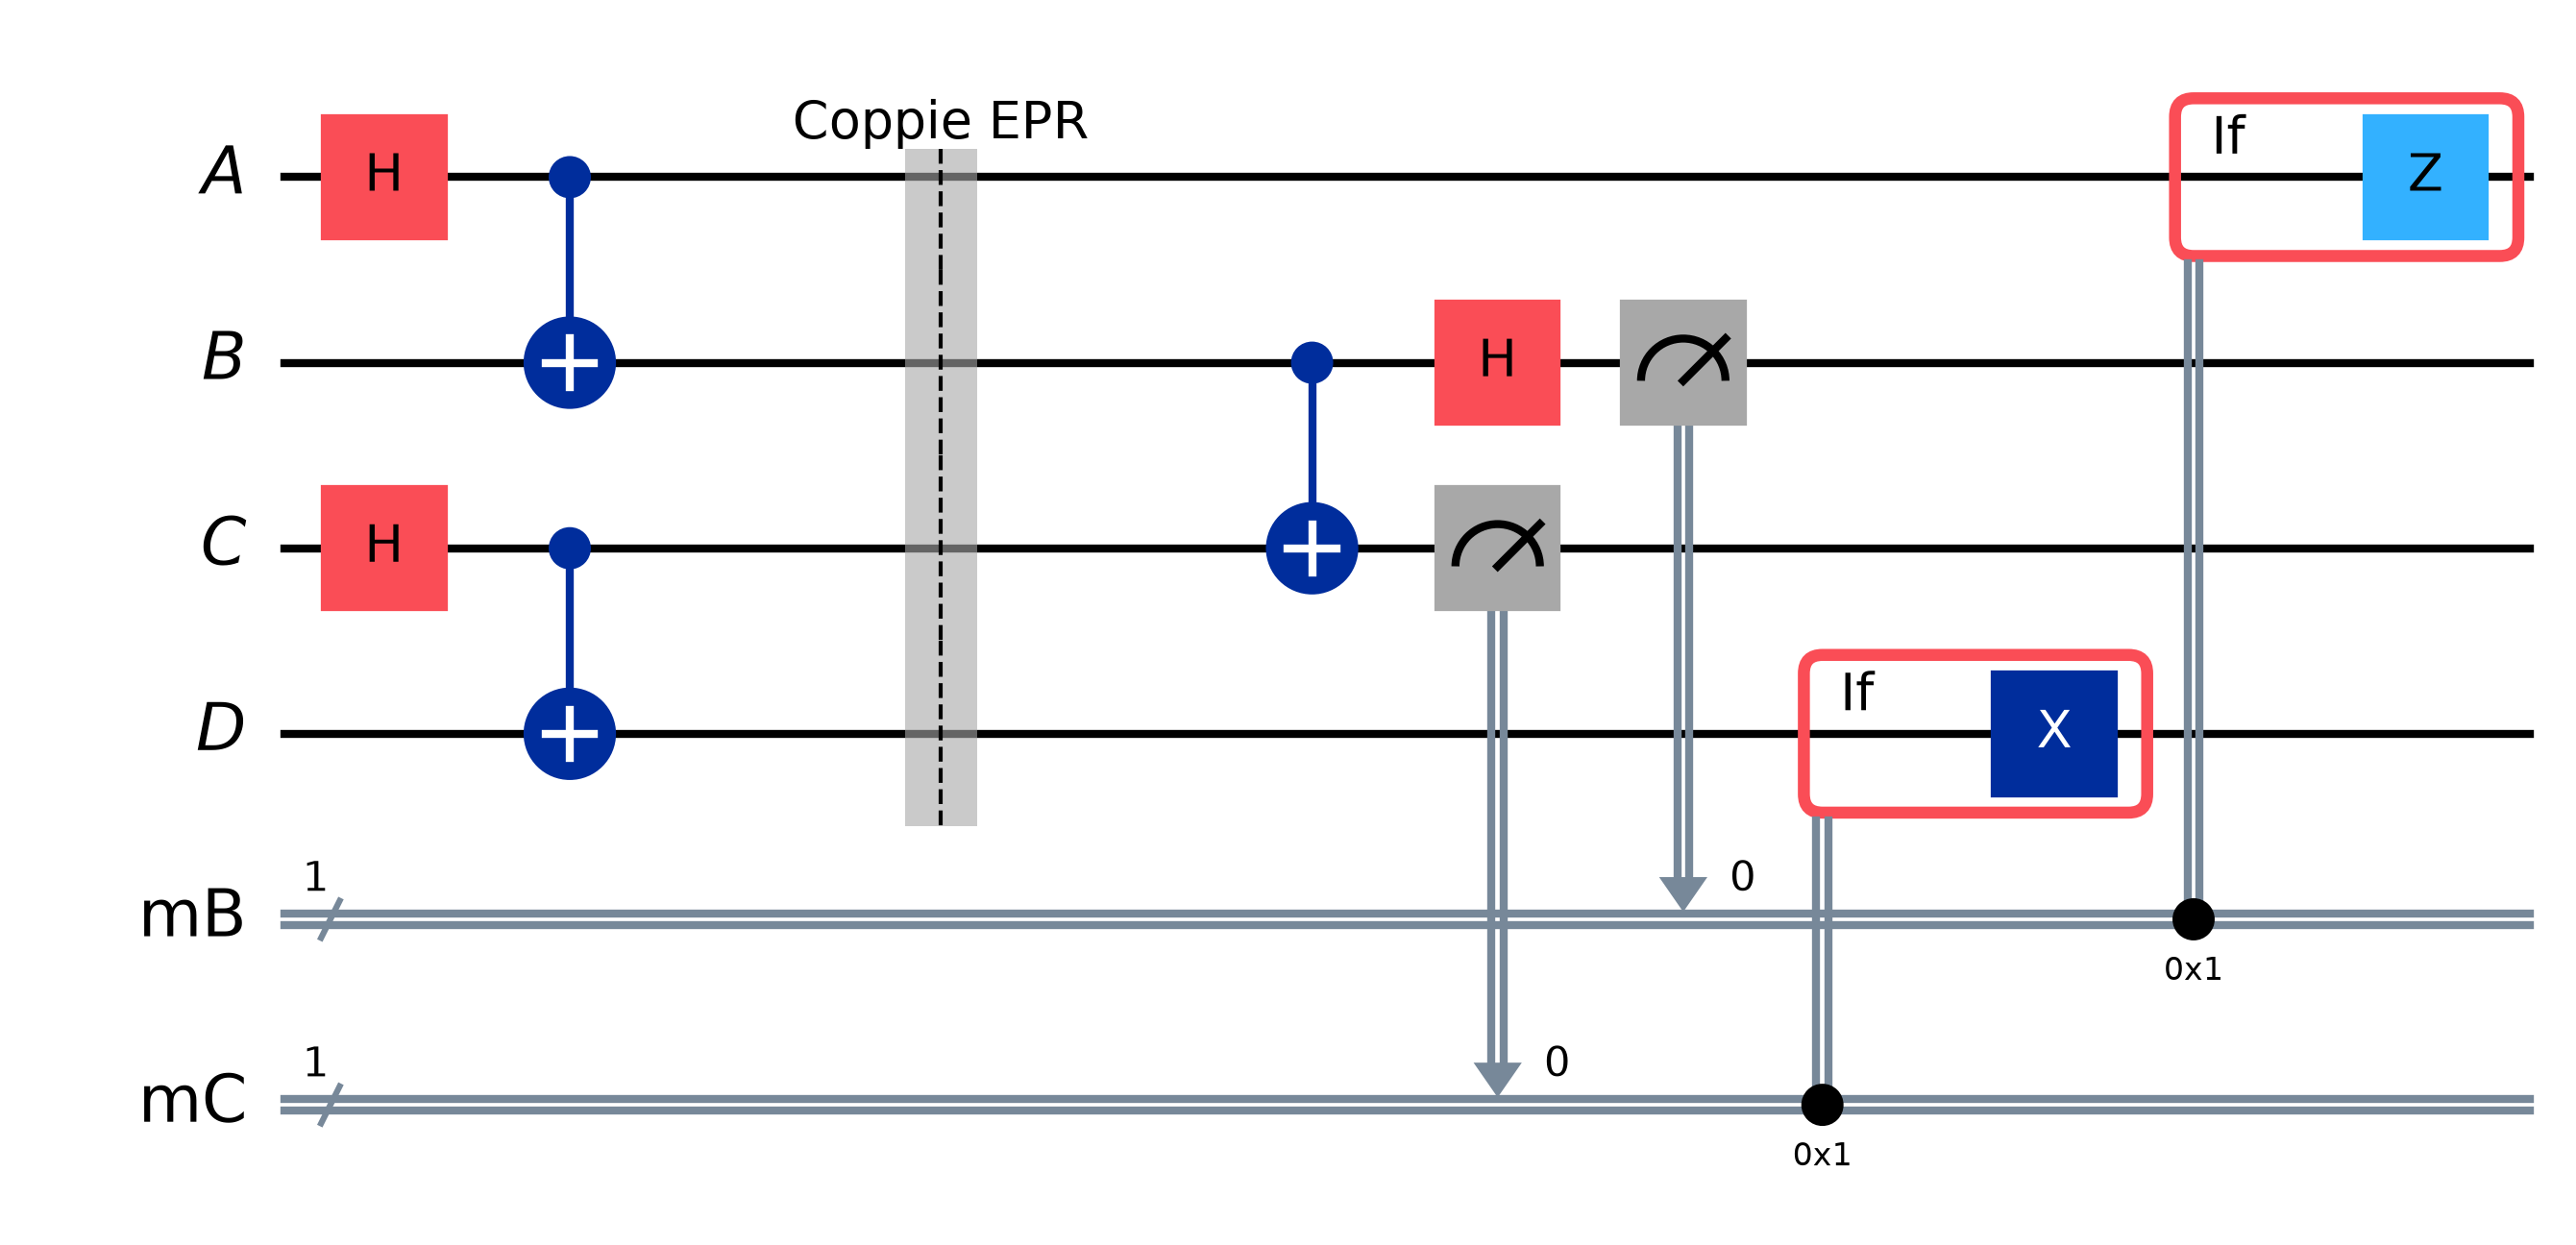
\includegraphics[width=\textwidth]{fig/Chapter-1/chapter-5/entanglement_swapping_misure.png}
\caption{Circuito dell'entanglement swapping}\label{img:ent-swapping}
\end{figure}

\subsection{Il paradosso dell'Entanglement}
Da quello che ci siamo detti prima, quindi, si potrebbe pensare che con una coppia di qubit entangled si possa trasferire informazione ad una velocità maggiore di quella della luce, ma questo non è proprio vero. Quando noi misuriamo su di una coppia EPR, il risultato è puramente probabilistico, il che va contro lo stesso significato di \textbf{informazione}, questo perchè il trasmettitore non decide cosa inviare al ricevitore, si avrà solo la certezza di aver misurato entrambi lo stesso stato, ma non che il trasmettitore volesse trasmettere effettivamente quello.

\begin{info}
\textbf{Significato di Condivisione dell'Informazione}\\
Condividere un informazione vuol dire che il ricevitore può risolvere una sua incertezza rispetto a quello che la sorgente vuole condividere.
Questo si ri-collega a quello che abbiamo detto precedentemente, ovvero, che se il mittente non può controllare cosa inviare, allora non si avrà un vero e proprio trasferimento di informazione, o almeno, non ad una velocità superiore a quella della luce
\end{info}

\subsection{Valutazione dell'entanglement in sistemi ad n-Qubit}
Il concetto di entanglement è fortemente legato al concetto di "decomposizione" del sistema, per capirci, se ho un sistema ad n-qubit, e non ci sono entanglement, io posso scrivere lo stato del sistema come:
\[
\ket{\psi} = \ket{\psi_0} \otimes \ket{\psi_1} \otimes \ket{\psi_3} \otimes \dots 
\]

Quindi come il prodotto tensoriale dei vari qubit appartenenti al mio sistema. Se vado a considerare i qubit accoappiati in coppie entangled, posso vederli come degli unici sistemi, potento poi ri-scrivere lo stato come:
\[
\ket{\psi} = \ket{wA} \otimes \ket{wB} \otimes \dots
\]

Dove \(\ket{wA}\) è l'entanglement tra 2 Qubit del sistema e \(\ket{wB}\) l'entanglement tra altri 2 ecc. 

Se guardassi il sistema in questo modo, potrei comunque esprimerlo come il prodotto vettoriale di tutte le coppie entanglate tra di loro. Nonostante questo, il sistema non sarebbe esprimibile come un prodotto tensoriale di tutti i qubit tra di loro. 

Questo discorso è importante per la definizione stessa che abbiamo dato di sistema in entanglement. Fino ad ora, se consideravamo due qubit il sistema risultava in entanglement perchè non potevo esprimerlo come prodotto tensoriale di due stati differenti, nel caso ad n-qubit, invece, dipende dal punto di vista. Se faccio un \textbf{clustering} rispetto ai singoli sistemi che sono in entanglement (come abbiamo fatto precedentemente considerando i due sistemi a 2 qubit come due sistemi separati e non entanglati tra di loro), allora posso esprimere lo stato del mio sistema come un prodotto vettoriale di questi ultimi. Quindi lo stato di entanglement di un sistema dipende anche in base a cosa voglio osservare ed agli entanglement "locali" tra i diversi qubit. 